\section{Breitensuche}


\begin{bem}
Die Eingabe für die Breitensuche ist ein Digraph $D=(V,A)$ in Form einer Adjazenzliste.
Auf ungerichteten Graphen ist die Vorgehensweise analog und wir diskutieren (fast ausschließlich) die gerichtete Variante.
\end{bem}

\begin{defn}
Für zwei Knoten $u,v \in V$ in~$D$ definieren wir den \emph{Abstand} von~$u$ nach~$v$ als die minimale Länge eines $(u,v)$-Pfades und bezeichnen ihn mit $\delta(u,v)$.
Wenn kein solcher Pfad existiert, setzen wir $\delta(u,v):=\infty$.
Für ungerichtete Graphen ist $\delta(u,v)$ entsprechend definiert und es gilt $\delta(u,v)=\delta(v,u)$ für alle Knoten $u,v \in V$.
Wie oben erwähnt erlaubt uns die Breitensuche das Bestimmen der Abstände $\delta(s,v)$ von einem festen \emph{Startknoten} $s \in V$ aus zu jedem anderen Knoten~$v$.
Ist $\delta(s,v) < \infty$, so sagen wir, dass~$v$ von~$s$ aus \emph{erreichbar} ist.
\end{defn} 

\begin{bem} 
Während der Durchmusterung des Digraphen~$D$ wird ein Array~$d$ der Länge~$|V|$ verwaltet, in dem nach Abschluss der Breitensuche die Abstände $\delta(s,v)$, für alle Knoten $v \in V$, gespeichert sind.
\end{bem} 

\begin{defn} 
Für die Umsetzung der Breitensuche wird die folgende Hilfsdatenstruktur benutzt.
Eine \emph{Warteschlange}~$Q$ ist eine Liste $Q=[q_1,\ldots,q_k]$, die mit zwei Grundoperationen ausgestattet ist:
\begin{itemize}
 \item $\cc{Dequeue}(Q)$: Das \emph{erste} Element~$q_1$ von~$Q$ wird zurückgegeben und aus der Warteschlange entfernt.
 Man nennt das Element~$q_1$ den \emph{Kopf} der Warteschlange und nach der Operation gilt $Q=[q_2,\ldots,q_k]$.

 \item $\cc{Enqueue}(Q,x)$: Das Element~$x$ wird am \emph{Ende} von~$Q$ hinzugefügt.
 Nach der Ausführung dieser Operation gilt also $Q=[q_1,\ldots,q_k,x]$. 
\end{itemize}
\end{defn} 

\begin{bem}
Aufgrund der Einfüge- und Rückgabereihenfolge sagt man auch, dass Warteschlangen nach dem FIFO-Prinzip (First In - First Out) arbeiten.
Warteschlangen mit höchstens $n \in \N$ Elementen können auf der Basis von Arrays der Länge~$n$ umgesetzt werden, sodass die Laufzeit der beiden Grundoperationen $\Theta(1)$ Zeiteinheiten beträgt. 
\end{bem} 

\begin{bem} 
Bevor wir mit der eigentlichen Breitensuche beginnen können, müssen eine Reihe von Attributen und natürlich auch die Warteschlange korrekt initialisiert werden:
Zu Beginn setzen wir $d[v]:=\infty$, für alle $v \in V \setminus \{s\}$, und $d[s]:=0$.
Besteht die Gleichheit $d[v]=\infty$ zu einem Moment der Breitensuche, so bedeutet dies, dass der Knoten~$v$ bisher noch nicht entdeckt wurde.
Die erste Veränderung des Wertes~$d[v]$ entspricht der Entdeckung von~$v$, und wir nennen $d[v]$ die \emph{aktuelle Distanz} von~$s$ zu~$v$. 
Wir verwalten weiterhin wie bei der Tiefensuche das Farbattribut $\cc{Farbe}[u]$ eines Knotens~$u \in V$ um den Bearbeitungszustand von~$u$ zu jedem Zeitpunkt der Breitensuche zu kennen.
Auch die Vorgängerabbildung~$\pi$ kommt wieder zum Einsatz.
\end{bem} 


\begin{bem} 
Wir fassen die Initialisierungen zu einer eigenen Hilfsprozedur zusammen:

\begin{algorithm}[H]
\caption{$\cc{Breitensuche-initialisieren}(D,s)$}
\begin{algorithmic}[1]
 \FOR{$u \in V \setminus \{s\}$}
  \STATE $\cc{Farbe}[u] := \cc{weiss}$
  \STATE $d[u] := \infty$ $\quad$ \COMMENT{Aktueller Abstand zu $s$}
  \STATE $\pi[u] := \cc{nil}$ $\quad$ \COMMENT{Vorgänger von $u$}
 \ENDFOR
 \STATE $\cc{Farbe}[s] := \cc{grau}$
 \STATE $d[s] := 0$
 \STATE $\pi[s] := \cc{nil}$
 \STATE Deklariere eine leere Warteschlange $Q$
 \STATE $\cc{Enqueue}(Q,s)$
\end{algorithmic}
\end{algorithm}
\end{bem}

\begin{bem}
Die Breitensuche ist so umgesetzt, dass das ``Leben'' eines jeden Knotens $u$ als der folgender Ablauf zusammengefasst werden kann: 
\begin{center}
	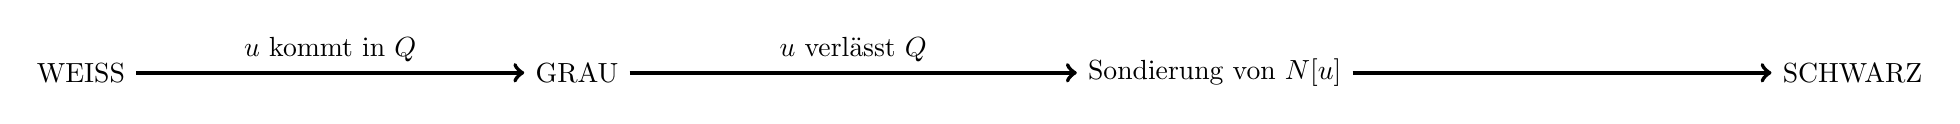
\begin{tikzpicture}[line width=1.5,scale=0.9] 
		\node (W) at (0,0) {WEISS} ;
		\node (G) at (7,0) {GRAU};
		\node(So) at (16,0) {Sondierung von $N[u]$} ;
		\node (S) at (25,0) {SCHWARZ};
		\draw[->] (W) edge node[above] {$u$ kommt in $Q$} (G) (G) edge node[above] {$u$ verlässt $Q$} (So) (So) edge (S);
	\end{tikzpicture} 
\end{center} 
Beim Sondieren von $N[u]$ werden werden weiße Knoten entdeckt: sie kommen in $Q$ und werden grau gefärbt. Die Breitensuche ist durch die Wahl des Containers $Q$ als Warteschlange ausgezeichnet. Durch diese Wahl ``simuliert'' die Breitensuche die Ausbreitung einer Welle in einem Medium. Stellen Sie sich vor: in $s$ kommt es zu einer Explosion; die Schallwelle breitet sich in $G$ entlang der Kanten aus und erreicht mit der Zeit immer mehr Knoten. Wie sich die Front der Schallwelle durch die Knoten ausbreitet wird durch die Warteschlange $Q$ ``modelliert''. 


\begin{algorithm}[H]
\caption{$\cc{Breitensuche}(s)$}
\begin{algorithmic}[1]
 \STATE $\cc{Breitensuche-initialisieren}(s)$
 \WHILE{$Q$ enthält Knoten}
  \STATE\label{line:breitensuche-dequeue} $u:=\cc{Dequeue}(Q)$ $\quad$ \COMMENT{Die Bearbeitung des Knotens $u$ beginnt.}
  \STATE \COMMENT{Aus $u$ ausgehende Kanten werden sondiert}
  \FOR{$v \in N[u]$}
   \IF{$\cc{Farbe}[v]=\cc{weiss}$}\label{line:breitensuche-if}
    \STATE $\cc{Farbe}[v]:=\cc{grau}$
    \STATE\label{line:breitensuche-enqueue} $\cc{Enqueue}(Q,v)$
    \STATE\label{line:breitensuche-pi} $\pi[v] := u$
    \STATE\label{line:breitensuche-d} $d[v]:=d[u]+1$
   \ENDIF
  \ENDFOR
  \STATE $\cc{Farbe}[u]:=\cc{schwarz}$
 \ENDWHILE
\end{algorithmic}
\end{algorithm}
\end{bem}

\begin{bsp}
\label{bsp:breitensuche}
Zum Vergleich mit der Tiefensuche sehen wir uns die Arbeitsweise der Breitensuche wieder auf dem Digaphen aus Beispiel~\ref{bsp:tiefensuche} an:

\hfill
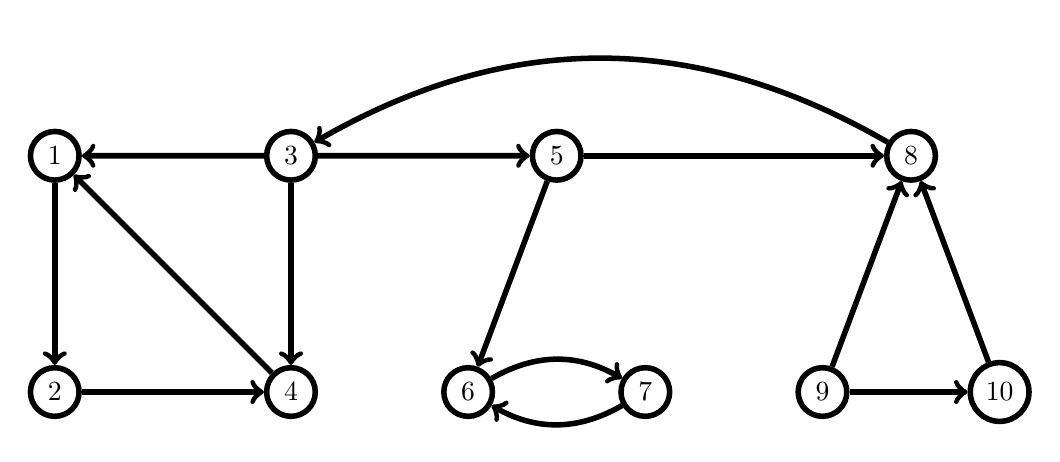
\begin{tikzpicture}[line width=2,scale=1.5]
 \node[circle,draw=black] (1) at (0,2) {$1$};
 \node[circle,draw=black] (2) at (0,0) {$2$};
 \node[circle,draw=black] (3) at (2,2) {$3$};
 \node[circle,draw=black] (4) at (2,0) {$4$};
 \node[circle,draw=black] (5) at (4.25,2) {$5$};
 \node[circle,draw=black] (6) at (3.5,0) {$6$};
 \node[circle,draw=black] (7) at (5,0) {$7$};
 \node[circle,draw=black] (8) at (7.25,2) {$8$};
 \node[circle,draw=black] (9) at (6.5,0) {$9$};
 \node[circle,draw=black] (10) at (8,0) {$10$};
		
 \draw[->] (1) edge (2);
 \draw[->] (2) edge (4);
 \draw[->] (3) edge (1) (3) edge (4) (3) edge (5);
 \draw[->] (4) edge (1);
 \draw[->] (5) edge (6) (5) edge (8); 
 \draw[->] (6) to[bend left] (7);
 \draw[->] (7) to[bend left] (6);
 \draw[->] (8) to[bend right] (3);
 \draw[->] (9) edge (8) (9) edge (10);
 \draw[->] (10) edge (8); 
\end{tikzpicture}
\hfill\,

Als Startknoten wählen wir wieder~$s=3$ und treffen ansonsten jede Wahl aufsteigend in der Reihenfolge der Knotenindizes.
Wir zeigen die ersten 8 Schritte und benutzen dieselbe Farbkodierung wie in Beispiel~\ref{bsp:tiefensuche}:

\hfill
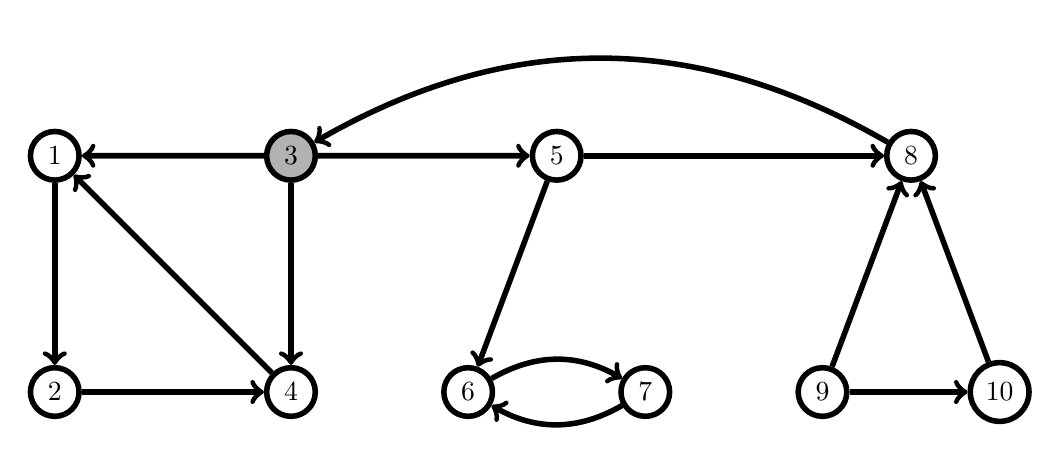
\begin{tikzpicture}[line width=2,scale=1.5]
 \tikzset{gnode/.style ={fill=black!30!,circle,draw}}
 \tikzset{snode/.style ={white,fill=black,circle,draw}}

 \node[circle,draw=black] (1) at (0,2) {$1$};
 \node[circle,draw=black] (2) at (0,0) {$2$};
 \node[gnode] (3) at (2,2) {$3$};
 \node[circle,draw=black] (4) at (2,0) {$4$};
 \node[circle,draw=black] (5) at (4.25,2) {$5$};
 \node[circle,draw=black] (6) at (3.5,0) {$6$};
 \node[circle,draw=black] (7) at (5,0) {$7$};
 \node[circle,draw=black] (8) at (7.25,2) {$8$};
 \node[circle,draw=black] (9) at (6.5,0) {$9$};
 \node[circle,draw=black] (10) at (8,0) {$10$};
		
 \draw[->] (1) edge (2);
 \draw[->] (2) edge (4);
 \draw[->] (3) edge (1) (3) edge (4) (3) edge (5);
 \draw[->] (4) edge (1);
 \draw[->] (5) edge (6) (5) edge (8); 
 \draw[->] (6) to[bend left] (7);
 \draw[->] (7) to[bend left] (6);
 \draw[->] (8) to[bend right] (3);
 \draw[->] (9) edge (8) (9) edge (10);
 \draw[->] (10) edge (8); 
\end{tikzpicture}
\hfill\,

\hfill
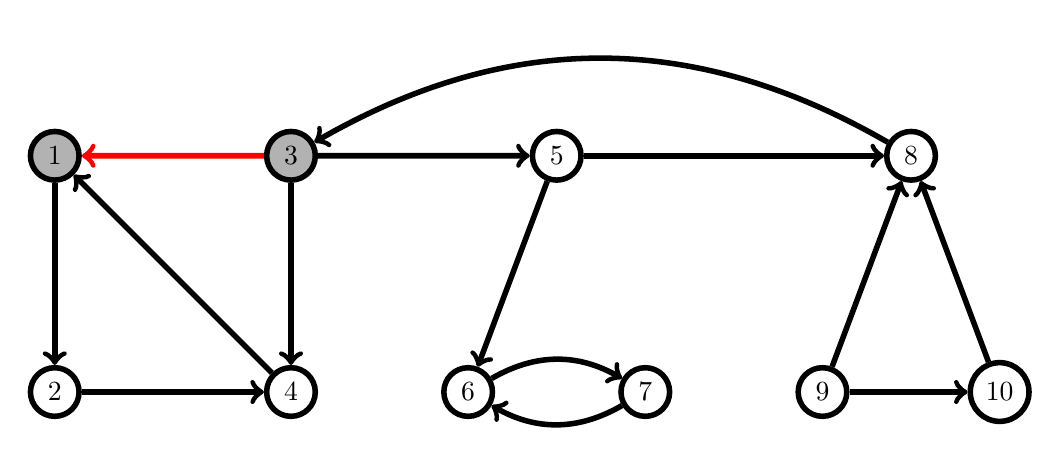
\begin{tikzpicture}[line width=2,scale=1.5]
 \tikzset{gnode/.style ={fill=black!30!,circle,draw}}
 \tikzset{snode/.style ={white,fill=black,circle,draw}}

 \node[gnode] (1) at (0,2) {$1$};
 \node[circle,draw=black] (2) at (0,0) {$2$};
 \node[gnode] (3) at (2,2) {$3$};
 \node[circle,draw=black] (4) at (2,0) {$4$};
 \node[circle,draw=black] (5) at (4.25,2) {$5$};
 \node[circle,draw=black] (6) at (3.5,0) {$6$};
 \node[circle,draw=black] (7) at (5,0) {$7$};
 \node[circle,draw=black] (8) at (7.25,2) {$8$};
 \node[circle,draw=black] (9) at (6.5,0) {$9$};
 \node[circle,draw=black] (10) at (8,0) {$10$};
		
 \draw[->] (1) edge (2);
 \draw[->] (2) edge (4);
 \draw[->,red] (3) edge (1);
 \draw[->] (3) edge (4) (3) edge (5);
 \draw[->] (4) edge (1);
 \draw[->] (5) edge (6) (5) edge (8); 
 \draw[->] (6) to[bend left] (7);
 \draw[->] (7) to[bend left] (6);
 \draw[->] (8) to[bend right] (3);
 \draw[->] (9) edge (8) (9) edge (10);
 \draw[->] (10) edge (8); 
\end{tikzpicture}
\hfill\,

\hfill
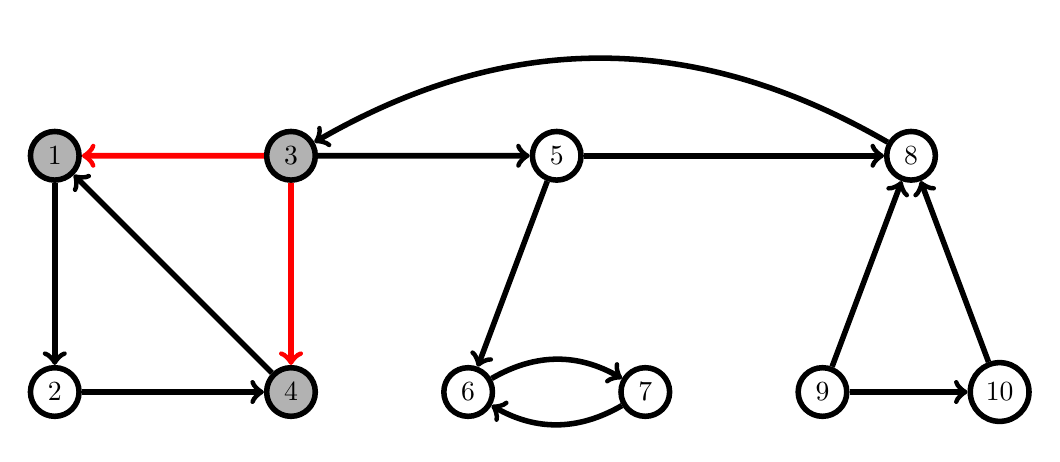
\begin{tikzpicture}[line width=2,scale=1.5]
 \tikzset{gnode/.style ={fill=black!30!,circle,draw}}
 \tikzset{snode/.style ={white,fill=black,circle,draw}}

 \node[gnode] (1) at (0,2) {$1$};
 \node[circle,draw=black] (2) at (0,0) {$2$};
 \node[gnode] (3) at (2,2) {$3$};
 \node[gnode] (4) at (2,0) {$4$};
 \node[circle,draw=black] (5) at (4.25,2) {$5$};
 \node[circle,draw=black] (6) at (3.5,0) {$6$};
 \node[circle,draw=black] (7) at (5,0) {$7$};
 \node[circle,draw=black] (8) at (7.25,2) {$8$};
 \node[circle,draw=black] (9) at (6.5,0) {$9$};
 \node[circle,draw=black] (10) at (8,0) {$10$};
		
 \draw[->] (1) edge (2);
 \draw[->] (2) edge (4);
 \draw[->,red] (3) edge (1);
 \draw[->,red] (3) edge (4);
 \draw[->] (3) edge (5);
 \draw[->] (4) edge (1);
 \draw[->] (5) edge (6) (5) edge (8); 
 \draw[->] (6) to[bend left] (7);
 \draw[->] (7) to[bend left] (6);
 \draw[->] (8) to[bend right] (3);
 \draw[->] (9) edge (8) (9) edge (10);
 \draw[->] (10) edge (8); 
\end{tikzpicture}
\hfill\,

\hfill
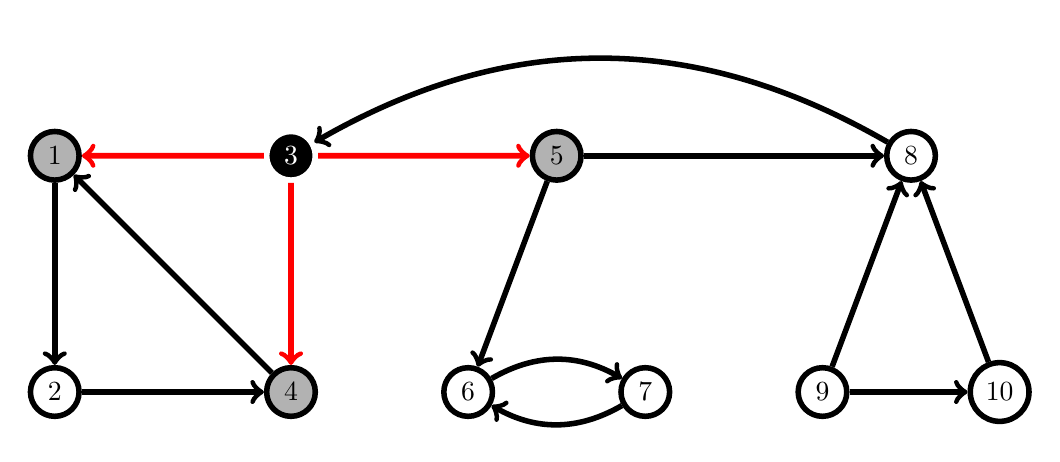
\begin{tikzpicture}[line width=2,scale=1.5]
 \tikzset{gnode/.style ={fill=black!30!,circle,draw}}
 \tikzset{snode/.style ={white,fill=black,circle,draw}}

 \node[gnode] (1) at (0,2) {$1$};
 \node[circle,draw=black] (2) at (0,0) {$2$};
 \node[snode] (3) at (2,2) {$3$};
 \node[gnode] (4) at (2,0) {$4$};
 \node[gnode] (5) at (4.25,2) {$5$};
 \node[circle,draw=black] (6) at (3.5,0) {$6$};
 \node[circle,draw=black] (7) at (5,0) {$7$};
 \node[circle,draw=black] (8) at (7.25,2) {$8$};
 \node[circle,draw=black] (9) at (6.5,0) {$9$};
 \node[circle,draw=black] (10) at (8,0) {$10$};
		
 \draw[->] (1) edge (2);
 \draw[->] (2) edge (4);
 \draw[->,red] (3) edge (1);
 \draw[->,red] (3) edge (4);
 \draw[->,red] (3) edge (5);
 \draw[->] (4) edge (1);
 \draw[->] (5) edge (6) (5) edge (8); 
 \draw[->] (6) to[bend left] (7);
 \draw[->] (7) to[bend left] (6);
 \draw[->] (8) to[bend right] (3);
 \draw[->] (9) edge (8) (9) edge (10);
 \draw[->] (10) edge (8); 
\end{tikzpicture}
\hfill\,

\hfill
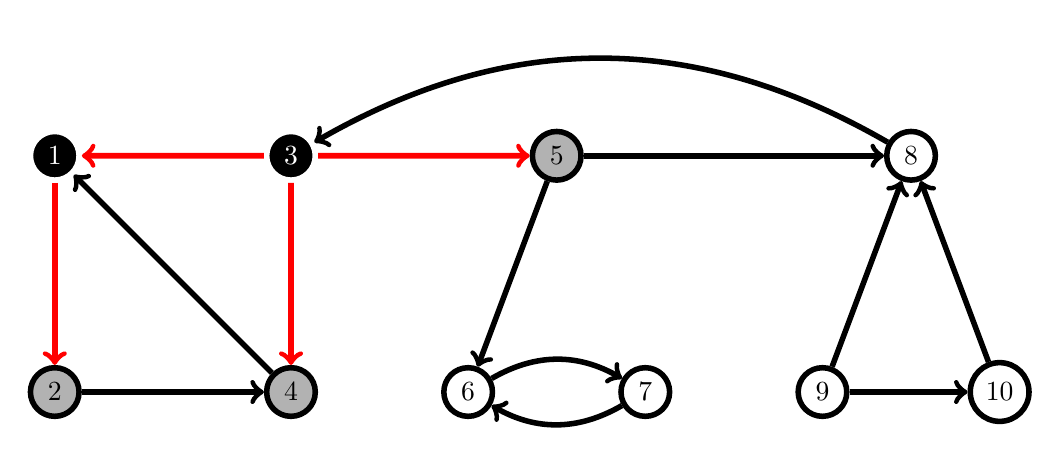
\begin{tikzpicture}[line width=2,scale=1.5]
 \tikzset{gnode/.style ={fill=black!30!,circle,draw}}
 \tikzset{snode/.style ={white,fill=black,circle,draw}}

 \node[snode] (1) at (0,2) {$1$};
 \node[gnode] (2) at (0,0) {$2$};
 \node[snode] (3) at (2,2) {$3$};
 \node[gnode] (4) at (2,0) {$4$};
 \node[gnode] (5) at (4.25,2) {$5$};
 \node[circle,draw=black] (6) at (3.5,0) {$6$};
 \node[circle,draw=black] (7) at (5,0) {$7$};
 \node[circle,draw=black] (8) at (7.25,2) {$8$};
 \node[circle,draw=black] (9) at (6.5,0) {$9$};
 \node[circle,draw=black] (10) at (8,0) {$10$};
		
 \draw[->,red] (1) edge (2);
 \draw[->] (2) edge (4);
 \draw[->,red] (3) edge (1);
 \draw[->,red] (3) edge (4);
 \draw[->,red] (3) edge (5);
 \draw[->] (4) edge (1);
 \draw[->] (5) edge (6) (5) edge (8); 
 \draw[->] (6) to[bend left] (7);
 \draw[->] (7) to[bend left] (6);
 \draw[->] (8) to[bend right] (3);
 \draw[->] (9) edge (8) (9) edge (10);
 \draw[->] (10) edge (8); 
\end{tikzpicture}
\hfill\,

\hfill
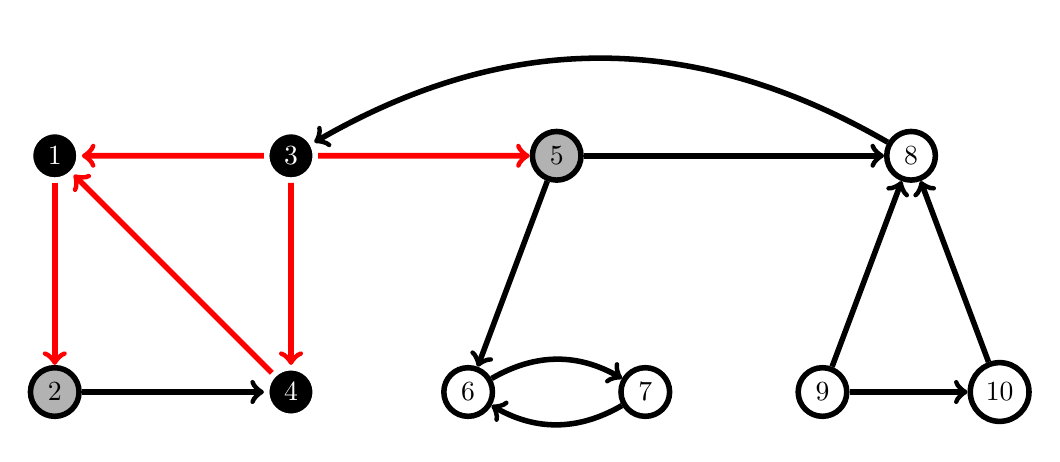
\begin{tikzpicture}[line width=2,scale=1.5]
 \tikzset{gnode/.style ={fill=black!30!,circle,draw}}
 \tikzset{snode/.style ={white,fill=black,circle,draw}}

 \node[snode] (1) at (0,2) {$1$};
 \node[gnode] (2) at (0,0) {$2$};
 \node[snode] (3) at (2,2) {$3$};
 \node[snode] (4) at (2,0) {$4$};
 \node[gnode] (5) at (4.25,2) {$5$};
 \node[circle,draw=black] (6) at (3.5,0) {$6$};
 \node[circle,draw=black] (7) at (5,0) {$7$};
 \node[circle,draw=black] (8) at (7.25,2) {$8$};
 \node[circle,draw=black] (9) at (6.5,0) {$9$};
 \node[circle,draw=black] (10) at (8,0) {$10$};
		
 \draw[->,red] (1) edge (2);
 \draw[->] (2) edge (4);
 \draw[->,red] (3) edge (1);
 \draw[->,red] (3) edge (4);
 \draw[->,red] (3) edge (5);
 \draw[->,red] (4) edge (1);
 \draw[->] (5) edge (6) (5) edge (8); 
 \draw[->] (6) to[bend left] (7);
 \draw[->] (7) to[bend left] (6);
 \draw[->] (8) to[bend right] (3);
 \draw[->] (9) edge (8) (9) edge (10);
 \draw[->] (10) edge (8); 
\end{tikzpicture}
\hfill\,

\hfill
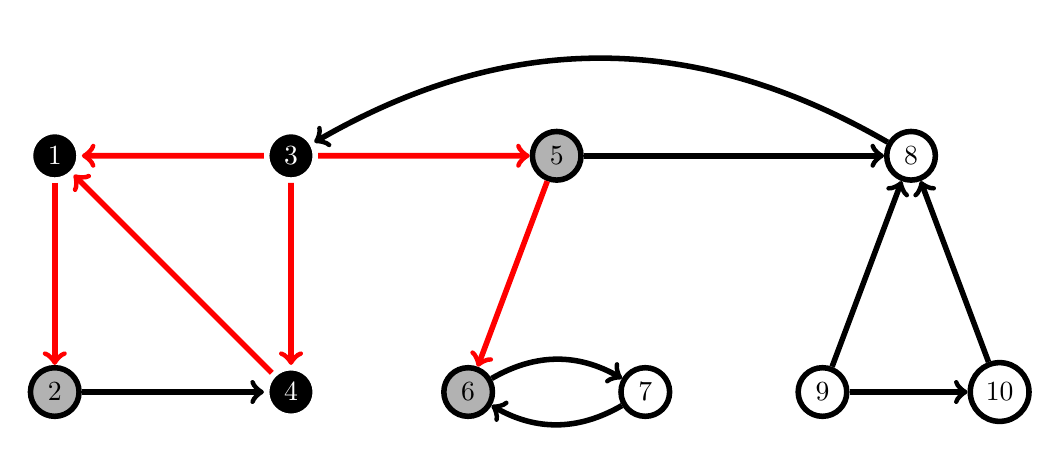
\begin{tikzpicture}[line width=2,scale=1.5]
 \tikzset{gnode/.style ={fill=black!30!,circle,draw}}
 \tikzset{snode/.style ={white,fill=black,circle,draw}}

 \node[snode] (1) at (0,2) {$1$};
 \node[gnode] (2) at (0,0) {$2$};
 \node[snode] (3) at (2,2) {$3$};
 \node[snode] (4) at (2,0) {$4$};
 \node[gnode] (5) at (4.25,2) {$5$};
 \node[gnode] (6) at (3.5,0) {$6$};
 \node[circle,draw=black] (7) at (5,0) {$7$};
 \node[circle,draw=black] (8) at (7.25,2) {$8$};
 \node[circle,draw=black] (9) at (6.5,0) {$9$};
 \node[circle,draw=black] (10) at (8,0) {$10$};
		
 \draw[->,red] (1) edge (2);
 \draw[->] (2) edge (4);
 \draw[->,red] (3) edge (1);
 \draw[->,red] (3) edge (4);
 \draw[->,red] (3) edge (5);
 \draw[->,red] (4) edge (1);
 \draw[->,red] (5) edge (6);
 \draw[->] (5) edge (8); 
 \draw[->] (6) to[bend left] (7);
 \draw[->] (7) to[bend left] (6);
 \draw[->] (8) to[bend right] (3);
 \draw[->] (9) edge (8) (9) edge (10);
 \draw[->] (10) edge (8); 
\end{tikzpicture}
\hfill\,

\hfill
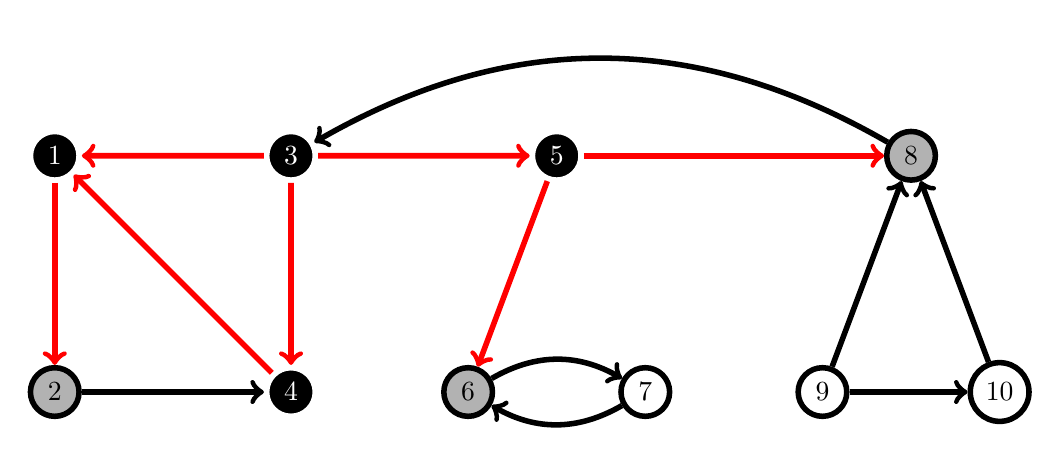
\begin{tikzpicture}[line width=2,scale=1.5]
 \tikzset{gnode/.style ={fill=black!30!,circle,draw}}
 \tikzset{snode/.style ={white,fill=black,circle,draw}}

 \node[snode] (1) at (0,2) {$1$};
 \node[gnode] (2) at (0,0) {$2$};
 \node[snode] (3) at (2,2) {$3$};
 \node[snode] (4) at (2,0) {$4$};
 \node[snode] (5) at (4.25,2) {$5$};
 \node[gnode] (6) at (3.5,0) {$6$};
 \node[circle,draw=black] (7) at (5,0) {$7$};
 \node[gnode] (8) at (7.25,2) {$8$};
 \node[circle,draw=black] (9) at (6.5,0) {$9$};
 \node[circle,draw=black] (10) at (8,0) {$10$};
		
 \draw[->,red] (1) edge (2);
 \draw[->] (2) edge (4);
 \draw[->,red] (3) edge (1);
 \draw[->,red] (3) edge (4);
 \draw[->,red] (3) edge (5);
 \draw[->,red] (4) edge (1);
 \draw[->,red] (5) edge (6) (5) edge (8); 
 \draw[->] (6) to[bend left] (7);
 \draw[->] (7) to[bend left] (6);
 \draw[->] (8) to[bend right] (3);
 \draw[->] (9) edge (8) (9) edge (10);
 \draw[->] (10) edge (8); 
\end{tikzpicture}
\hfill\,

Da die Knoten~$9$ und~$10$ nicht vom Startknoten $s=3$ aus erreichbar sind, ist der Endzustand nach dem Abschluss von $\cc{Breitensuche}(3)$ der folgende:

\hfill
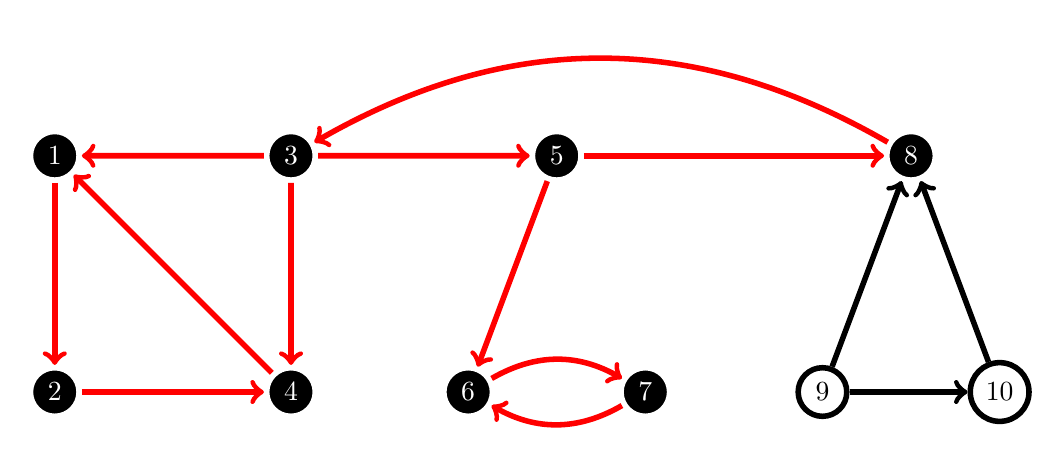
\begin{tikzpicture}[line width=2,scale=1.5]
 \tikzset{gnode/.style ={fill=black!30!,circle,draw}}
 \tikzset{snode/.style ={white,fill=black,circle,draw}}

 \node[snode] (1) at (0,2) {$1$};
 \node[snode] (2) at (0,0) {$2$};
 \node[snode] (3) at (2,2) {$3$};
 \node[snode] (4) at (2,0) {$4$};
 \node[snode] (5) at (4.25,2) {$5$};
 \node[snode] (6) at (3.5,0) {$6$};
 \node[snode] (7) at (5,0) {$7$};
 \node[snode] (8) at (7.25,2) {$8$};
 \node[circle,draw=black] (9) at (6.5,0) {$9$};
 \node[circle,draw=black] (10) at (8,0) {$10$};
		
 \draw[->,red] (1) edge (2);
 \draw[->,red] (2) edge (4);
 \draw[->,red] (3) edge (1);
 \draw[->,red] (3) edge (4) (3) edge (5);
 \draw[->,red] (4) edge (1);
 \draw[->,red] (5) edge (6) (5) edge (8); 
 \draw[->,red] (6) to[bend left] (7);
 \draw[->,red] (7) to[bend left] (6);
 \draw[->,red] (8) to[bend right] (3);
 \draw[->] (9) edge (8) (9) edge (10);
 \draw[->] (10) edge (8); 
\end{tikzpicture}
\hfill\,
\end{bsp}

\begin{bem}
Der Beweis der Korrektheit der Breitensuche inklusive der korrekten Bestimmung der Abstände $\delta(s,v)$, für $v \in V$, erfordert noch etwas Vorbereitung.
Die Laufzeitanalyse können wir allerdings bereits durchführen, mit dem Ergebnis, dass auch die Breitensuche einen optimalen linearen Aufwand erfordert:
\end{bem}

\begin{thm}
\label{thm:laufzeit-breitensuche}
Es sei ein Digraph $D=(V,A)$ durch eine Adjazenzliste gegeben und es sei $s \in V$ ein beliebiger Startknoten.
Die Laufzeit von $\cc{Breitensuche}(s)$ ist $\Theta(|V|+|A|)$.
\end{thm}

\begin{proof}
Der Aufwand für die Initialisierung $\cc{Breitensuche-initialisieren}(D,s)$ ist direkt als $\Theta(|V|)$ festzustellen. Der Aufwand von $\cc{Breitensuche}(s)$ kann aus dem Diagramm zur Bearbeitung von Knoten $u \in V$ abgelesen werden: 
\vspace{1ex}
\begin{center}
	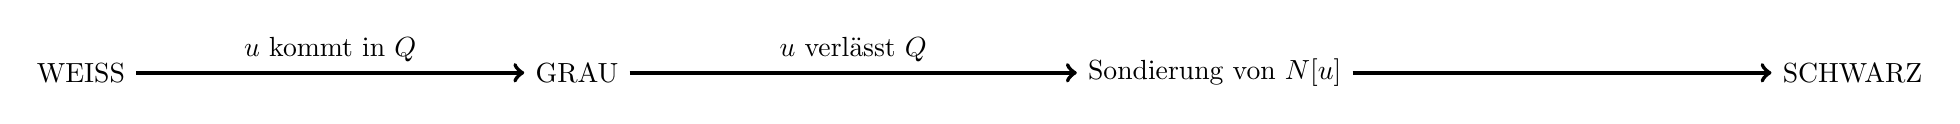
\begin{tikzpicture}[line width=1.5,scale=0.9] 
		\node (W) at (0,0) {WEISS} ;
		\node (G) at (7,0) {GRAU};
		\node(So) at (16,0) {Sondierung von $N[u]$} ;
		\node (S) at (25,0) {SCHWARZ};
		\draw[->] (W) edge node[above] {$u$ kommt in $Q$} (G) (G) edge node[above] {$u$ verlässt $Q$} (So) (So) edge (S);
	\end{tikzpicture} 
\end{center} 
Der Aufwand pro Knoten, der entdeckt wird ist konstant: der Aufwand  besteht aus der Aufnahme in $Q$,  der Färbung von Weiß zu Grau und von Grau zu Schwarz. Der Aufwand pro Kante $(u,v)$, die sondiert wird, ist ebenfalls konstant: jede Kante $(u,v)$ wird höchstens ein mal sondiert, denn die Sondierung erfolgt nach der Entfernung von $u$ aus der Warteschlange. Nach der Entfernung von $u$ wird $u$ schwarz gefärbt und daher nicht mehr in $Q$ aufgenommen. 

Zusammenfassend erhalten wir also  wie behauptet einen Zeitaufwand von $\Theta(|V|) + \Theta(|V|) + \Theta(|A|) = \Theta(|V|+|A|)$.
\end{proof}


\begin{defn}
Wir nennen einen $(s,v)$-Pfad der Länge $\delta(s,v)$ einen \emph{kürzesten Pfad} von~$s$ nach~$v$ in~$D$.
\end{defn}

\begin{lem}
\label{lem:breitensuche-pfad-dreieck}
Sei $D=(V,A)$ ein Digraph und sei $s \in V$ ein beliebiger Startknoten.
Dann gilt für jede Kante $(u,v) \in A$, dass
\[
\delta(s,v) \leq \delta(s,u) + 1.
\]
\end{lem}

\begin{proof}
Falls $u$ von $s$ aus erreichbar ist, dann ist es auch~$v$.
In diesem Fall ist der kürzeste $(s,v)$-Pfad nicht länger als der kürzeste $(s,u)$-Pfad, verlängert um die Kante $(u,v)$, und die Ungleichung gilt.
Ist~$u$ nicht von~$s$ aus erreichbar, so ist $\delta(s,u)=\infty$, und die Ungleichung ist trivialerweise erfüllt.
\end{proof}

\begin{lem}
\label{lem:breitensuche-d-geq-delta}
Sei $D=(V,A)$ ein Digraph und sei $s \in V$ ein beliebiger Knoten.
Nach Abschluss der Prozedur $\cc{Breitensuche}(s)$ gilt $d[v] \geq \delta(s,v)$, für alle $v \in V$.
\end{lem}

\begin{proof}
Wir argumentieren mittels vollständiger Induktion nach der Anzahl der Ein\-füge\-operationen in die Warteschlange~$Q$.

Der Induktionsanfang ist der Zeitpunkt nach der Initialisierung zu dem $d[s]=0=\delta(s,s)$ und, für alle $v \in V \setminus \{s\}$, die Ungleichung $d[v]=\infty\geq\delta(s,v)$ gilt.

Für den Induktionsschritt sei~$v$ ein weißer Knoten, der bei der Suche vom Knoten~$u$ aus entdeckt wird.
Nach Induktionsvoraussetzung gilt $d[u] \geq \delta(s,u)$.
Aufgrund der Zuweisung in Zeile~\ref{line:breitensuche-d} in $\cc{Breitensuche}(s)$ und Lemma~\ref{lem:breitensuche-pfad-dreieck} gilt
\[
d[v] = d[u] + 1 \geq \delta(s,u) + 1 \geq \delta(s,v).
\]
Der Knoten~$v$ wird in die Warteschlange~$Q$ eingefügt, und da er zu diesem Zeitpunkt grau gefärbt wurde, ändert sich der Wert $d[v]$ nicht mehr und die Ungleichung bleibt bis zur Terminierung des Algorithmus gültig.
\end{proof}

\begin{bem} 
Wir fassen dafür die Warteschlange als Liste oder Array $[v_1,\ldots,v_r]$ auf, wobei $v_1$ der Kopf und $v_r$ das Ende von~$Q$ ist.
\end{bem} 

\begin{lem}
\label{lem:breitensuche-warteschlange-monotonie}
Zu jedem Zeitpunkt der Ausführung von $\cc{Breitensuche}(s)$ erfüllt die Warteschlange $Q=[v_1,\ldots,v_r]$ die Bedingung
\[
d[v_1] \leq d[v_2] \leq \ldots \leq d[v_r] \leq d[v_1] + 1.
\]
Mit anderen Worten: die Liste 
\[
	Q_d:=[d[v_1],\ldots,d[v_r]]
\] der Distanzen der Knoten von $Q$ hat die Form $[t,\ldots,t]$ oder die Form $[t,\ldots,t,t+1,\ldots,t+1]$ mit $t \in \N_0$ (die Liste $Q_d$ enthält einen Wert oder zwei aufeinanderfolgende ganzzahlige Werte und sie ist aufsteigend sortiert). 
\end{lem}

\begin{proof}
Ganz am Anfang der Breitensuche enthält~$Q$ nur den Startknoten~$s$ und die Aussage gilt trivialerweise.

Wir zeigen, dass wenn die behauptete Bedingung zu einem Zeitpunkt gilt, dass sie auch dann gültig bleibt, wenn eine Warteschlangenoperation ausgeführt wird.
(Das heißt, wir argumentieren mittels vollständiger Induktion über die Anzahl der ausgeführten Warteschlangenoperationen.)

\condclearpage 

Sei zunächst wie angenommen $Q=[v_1,\ldots,v_r]$ und führen wir $\cc{Dequeue}(Q)$ aus.
Hat die Liste $Q_d$ die Form $[t,\ldots,t]$ so, hat sie nach der Entfernung von $v_1$ immer noch die Form $[t,\ldots,t]$ (und Länge um eins kleiner).  Hat die Liste $Q_d$ die Form $[t,\ldots,t,t+1,\ldots,t+1]$ so, hat hat sie nach der Entfernung von $v_1$ die Form $[t,\ldots,t,t+1,\ldots,t+1]$ mit dem Block $t,\ldots,t$, dessen Länge um eins geringer geworden ist, oder die Form $[t+1,\ldots,t+1]$. 

\condclearpage 

Schauen wir uns an, was passiert, wenn in Zeile~\ref{line:breitensuche-enqueue} von $\cc{Breitensuche}(s)$ die Operation $\cc{Enqueue}(Q,v)$ ausgeführt wird.
Der Knoten~$v$ wird zum Ende der neuen Warteschlange $Q'=[v_1,\ldots,v_r,v]$ und zum Zeitpunkt dieser Operation durchsucht der Algorithmus die Nachbarschaft des Knotens~$u$, der zuvor aus der Warteschlange entfernt wurde.
Daher gilt nach Annahme die Ungleichung $d[u] \leq d[v_i]$ für alle $1 \leq i \leq r$ und nach Zeile~\ref{line:breitensuche-d} weiterhin $d[v] = d[u]+1 \leq d[v_1]+1$.
Es gilt außerdem, dass $d[v_r] \leq d[u]+1=d[v]$, da wie bereits erwähnt, $u$ zuvor aus der Schlange entfernt wurde, und nach Annahme die Aussage des Lemmas vor der Operation $\cc{Enqueue}(Q,v)$ gilt.
Alle anderen Ungleichungen bleiben unangetastet und wir erhalten zusammenfassend
\[
d[v_1] \leq d[v_2] \leq \ldots d[v_r] \leq d[v] \leq d[v_1] + 1,
\]
wie gewünscht.
\end{proof}

\begin{kor}
\label{cor:breitensuche-warteschlange}
Seien $v'$ und $v''$ Knoten die während der Ausführung von $\cc{Breitensuche}(s)$ in $Q$ eingefügt werden, und nehmen wir weiterhin an, dass~$v'$ vor $v''$ eingefügt wird.
Dann gilt $d[v'] \leq d[v'']$ zum Zeitpunkt des Einfügens von~$v''$.
\end{kor}

\begin{proof}
Aus Lemma~\ref{lem:breitensuche-warteschlange-monotonie} folgt: solange $Q$ nicht leer ist, wächst das Maximum von $Q_d$ monoton während der Ausführung der Breitensuche (monotones Wachstum im nicht-strikten Sinn). Die Entfernung des Kopfs verändert $Q_d$ nicht, solange die Schlange $Q$ nicht leer ist. Beim Hinzufügen eines neuen Elements zu $Q$ bleibt das Maximum im Fall $Q_d=[t,\ldots,t,t+1,\ldots,t+1]$ unverändert und es wächst um eine Einheit bei $Q_d=[t,\ldots,t]$, weil nach dem Hinzufügen $Q_d = [t,\ldots,t,t+1]$ ist. 
\end{proof}



\begin{thm}
\label{thm:breitensuche}
Sei $D=(V,A)$ ein Digraph und sei $s \in V$ ein beliebiger Knoten.
Dann entdeckt die Prozedur $\cc{Breitensuche}(s)$ während ihrer Ausführung jeden Knoten, der von~$s$ aus erreichbar ist, und bei der Terminierung gilt $d[v] = \delta(s,v)$, für alle $v \in V$.

Außerdem besteht für jeden von~$s$ aus erreichbaren Knoten $v \neq s$, einer der kürzesten $(s,v)$-Pfade aus einem kürzesten $(s,\pi[v])$-Pfad und der Kante $(\pi[v],v)$.
\end{thm}

\begin{proof}
Wir führen einen Widerspruchsbeweis und nehmen dazu an, dass es einen Knoten~$v$ gibt, so dass $d[v] \neq \delta(s,v)$ gilt.
Sei weiterhin angenommen, dass~$v$ ein solcher Knoten mit kleinstem Abstand $\delta(s,v)$ zu~$s$ ist.
Da $d[s]=0=\delta(s,s)$ gilt, ist demnach in jedem Fall $v \neq s$.
Nach Lemma~\ref{lem:breitensuche-d-geq-delta} ist $d[v] \geq \delta(s,v)$ und daher $d[v] > \delta(s,v)$ für diesen ausgezeichneten Knoten~$v$.
Weiterhin muss~$v$ von~$s$ aus erreichbar sein, da ansonsten $\delta(s,v)=\infty \geq d[v]$ gelte.
Sei nun~$u$ ein Knoten auf einem kürzesten $(s,v)$-Pfad, der unmittelbar vor~$v$ liegt, so dass $\delta(s,v)=\delta(s,u)+1$ gilt.
Die Wahl des Knotens~$v$ zusammen mit $\delta(s,u) < \delta(s,v)$ ergibt die Identität $d[u]=\delta(s,u)$, und wir fassen unsere Beobachtungen in folgender Ungleichungskette zusammen
\begin{align}
d[v] &> \delta(s,v) = \delta(s,u) + 1 = d[u] + 1.\label{eqn:breitensuche-korrekt}
\end{align}

Sehen wir uns den Zeitpunkt an, zu dem der Algorithmus $\cc{Breitensuche}(s)$ in Zeile~\ref{line:breitensuche-dequeue} den Knoten~$u$ aus der Warteschlange entfernt.
Wir unterscheiden danach, welche Farbe $\cc{Farbe}[v]$ der Knoten~$v$ zu diesem Zeitpunkt trägt:

Ist $\cc{Farbe}[v]=\cc{weiss}$, so wird in Zeile~\ref{line:breitensuche-d} $d[v]=d[u]+1$ gesetzt und danach im Algorithmus nicht mehr verändert.
Dies steht im Widerspruch zu~\eqref{eqn:breitensuche-korrekt}.

Ist $\cc{Farbe}[v]=\cc{grau}$, so ist $v$ beim Sondieren eines anderen Knotens~$w$  grau gefärbt worden.
Dieser Knoten wurde früher als~$u$ aus der Warteschlange entfernt und es wurde $d[v]=d[w]+1$ gesetzt.
Nach Korollar~\ref{cor:breitensuche-warteschlange} gilt daher $d[w] \leq d[u]$ und damit $d[v]=d[w]+1 \leq d[u]+1$, im Widerspruch zu~\eqref{eqn:breitensuche-korrekt}.

Ist $\cc{Farbe}[v]=\cc{schwarz}$, so wurde~$v$ bereits aus der Warteschlange entfernt und nach Korollar~\ref{cor:breitensuche-warteschlange} gilt $d[v] \leq d[u]$, im Widerspruch zu~\eqref{eqn:breitensuche-korrekt}.

Zusammenfassend erhalten wir in jedem Fall einen Widerspruch zu~\eqref{eqn:breitensuche-korrekt} und damit gilt also $d[v]=\delta(s,v)$, für alle Knoten $v \in V$.

Alle von~$s$ aus erreichbaren Knoten werden bei der Breitensuche entdeckt, da für einen ansonsten unentdeckten Knoten~$v$ der Initialwert $d[v]=\infty$ größer als $\delta(s,v)$ wäre.
Abschließend bemerken wir noch, dass die Verwaltung der Vorgängerabbildung~$\pi$ und des Abstandsattributs~$d$ in den Zeilen~\ref{line:breitensuche-pi} und~\ref{line:breitensuche-d} von $\cc{Breitensuche}(s)$ impliziert, dass $\delta(s,v)=d[v]=d[\pi[v]]+1=\delta(s,\pi[v])+1$ gilt und somit jeder kürzeste $(s,\pi[v])$-Pfad über die Kante $(\pi[v],v)$ zu einem kürzesten $(s,v)$-Pfad erweitert werden kann.
\end{proof}

\begin{defn} 
	Die Vorgängerabbildung $\pi$ aus der Breitensuche erzeugt auf einem Digraphen $D=(V,A)$, die von einem Startknoten~$s \in V$ ausgeht, einen \emph{Vorgängerteilgraphen} $D_\pi = (V_\pi,A_\pi)$, der durch
	\[
	V_\pi := \left\{ v \in V : \pi[v] \neq \cc{nil}\right\} \cup \{s\} \quad \text{ und } \quad A_\pi := \left\{ (\pi[v],v) : v \in V_\pi \setminus \{s\}\right\}
	\]
	definiert ist.
	
	Es kann gezeigt, werden dass $D_\pi$ ein gerichteter Baum mit Wurzel $s$ ist. Dieser Baum nennt man den \textbf{Breitensuchbaum} der Breitensuche. die  Kanten von $D_\pi$ werden die \textbf{Baumkanten} der Breitensuche genannt.
\end{defn}

\begin{bem}Zur Berechnung der kürzesten Pfade kann die folgende Prozedur benutzt werden: 
	\begin{algorithm}[H]
	\caption{$\cc{Pfad-Ausgeben}(v)$}
	\begin{algorithmic}[1]
		\IF{$v=s$}
		\STATE print $s$
		\ELSE
		\STATE $\cc{Pfad-Ausgeben}(s,\pi[v])$
		\STATE print $v$
		\ENDIF
	\end{algorithmic}
\end{algorithm}
\end{bem}

\begin{prop}
	Ist $\pi$ die Vorgängerabbildung zur Breitensuche auf $G=(V,A)$ mit dem Startknoten $s$, so gibt die Prozedur $\cc{Pfad-Ausgeben}(v)$ folgende Algorithmus für jedes $v \in V$ mit $\delta(s,v)<\infty$ einen kürzesten $(s,v)$-Pfad aus. 
\end{prop}
\begin{proof} 
Außerdem wissen wir, dass nach der Terminierung der Breitensuche $d[v]=\delta(s,v)$ für alle $v \in V$ gilt. Dass die Prozedur $\cc{Pfad-Ausgeben}(v)$ terminiert und einen kürzesten $(s,v)$-Pfad ausgibt kann durch Induktion über $\delta(s,v)$ gezeigt werden. ist $\delta(s,v)=0$ so ist $v=0$ und die Behauptung ist klar. Angenommen, die Behauptung gelte für alle $v \in V$ mit $\delta(s,v)=t-1$ für ein $t \in \N$. 

Wir betrachten ein $v \in V$ mit $\delta(s,v)$. 	In der Breitensuche setzt man  $\pi[v] := u$ gleichzeitig mit $d[v] = d[u]+1$ für $v \in N[u]$. Daher hat man $t = d[v] = d[\pi[u]] + 1 $, sodass $d[\pi[u]]=t-1$ gilt. Nach der Induktionsvoraussetzung  gibt $\cc{Pfad-Ausgeben}(s,\pi[v])$ den $(s,\pi[v])$-Pfad der Lange $\delta(s,\pi[u]) = d[\pi[u]]  = t-1$ aus. Also gibt $\cc{Pfad-Ausgeben}(v)$ den $(s,v)$-Pfad der Länge $t = d[v] = \delta(s,v)$ aus, was die Korrektheit und die Terminierung der Ausführung Prozedur $\cc{Pfad-Ausgeben}$  auf dem Knoten $v$ bestätigt. 
\end{proof} 



\begin{bsp}
Sammeln wir die Daten zur Vorgängerabbildung und zu den Distanzen während der Breitensuche in Beispiel~\ref{bsp:breitensuche}, so erhalten wir nach Abschluss von $\cc{Breitensuche}(3)$ die folgenden Werte:

\begin{table}[H]
\centering
\begin{tabular}{|c|c|c|c|c|c|c|c|c|c|c|}
\hline
\textbf{Knoten $u$}        & \textbf{1} & \textbf{2} & \textbf{3} & \textbf{4} & \textbf{5} & \textbf{6} & \textbf{7} & \textbf{8} & \textbf{9} & \textbf{10} \\ \hline
\textbf{$\pi[u]$}    & 3          & 1          & $\cc{nil}$          & 3          & 3          & 5          & 6         & 5         & $\cc{nil}$         & $\cc{nil}$          \\ \hline
\textbf{$d[u]$} & 1          & 2          & 0         & 1          & 1         & 2         & 3         & 2         & $\infty$         & $\infty$          \\ \hline
\end{tabular}
\end{table}

Daraus ergibt sich der nachfolgende Breitensuchbaum, in dem der kürzeste $(3,7)$-Pfad in blau markiert ist:

\begin{center} 
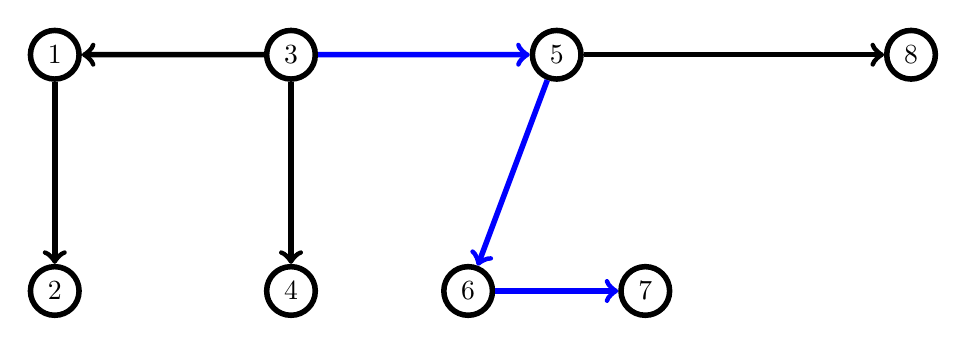
\begin{tikzpicture}[line width=2,scale=1.5]
 \node[circle,draw=black] (1) at (0,2) {$1$};
 \node[circle,draw=black] (2) at (0,0) {$2$};
 \node[circle,draw=black] (3) at (2,2) {$3$};
 \node[circle,draw=black] (4) at (2,0) {$4$};
 \node[circle,draw=black] (5) at (4.25,2) {$5$};
 \node[circle,draw=black] (6) at (3.5,0) {$6$};
 \node[circle,draw=black] (7) at (5,0) {$7$};
 \node[circle,draw=black] (8) at (7.25,2) {$8$};
% \node[circle,draw=black] (9) at (6.5,0) {$9$};
% \node[circle,draw=black] (10) at (8,0) {$10$};
		
 \draw[->] (1) edge (2);
 \draw[->] (3) edge (4);
 \draw[->] (3) edge (1) ;
 \draw[->] (5) edge (8); 
 \draw[->,blue] (3) edge (5) (5) edge (6) (6) edge (7);
\end{tikzpicture}
\end{center} 

Beachten Sie, dass die Knoten $9$ und $10$ nicht im Breitensuchbaum auftreten, da diese vom Startknoten~$s=3$ aus nicht erreichbar sind.
\end{bsp}

\begin{bem}
	Die Präsentation der Breitensuche hier basiert auf \cite{CLRS17}. 
\end{bem} 
